\chapter{Konzeption}

\section{Bewertungskriterien}
 
 Im folgenden Kapitel werden drei Lösungsalternativen zur mobilen Aufmaßerfassung aus dem Google Play-Store anhand der erweiterteten Nielsen-Heuristiken \todo{ref} bewertet und verglichen.
Hierzu werden die Heuristiken zunächst kurz vorgestellt, und anschließend iterativ auf die Apps angewendet. Die für den Einsatzbereich des Gerüstbaus am Wichtigsten Kriterien werden abschließend in einer vergleichenden Tabelle zusammengetragen, um einen guten Überblick über die Testergebnisse zu schaffen. \\

 Diese drei ausgewählten Apps waren bei der Suchanfrange nach ``Aufmaßerfassung'' im Play-Store die am best bewerteten (Stand Januar 2018)
 \todo{Bild vom play-store} \\
 
 
 \subsection{Erweiterte Nielsen-Heuristiken}
 Nach \citeauthor{Nielsen:1994:UIM} gibt es 10 Heuristiken, die auf einer Grundlage von allgemein anerkannten Prinzipien beruhen, und sich zur Evaluation von Usability-Problemen gut eignen \citep[Seite.~25--62]{Nielsen:1994:UIM}: 

\begin{enumerate}
	\item \label{itm:1} Sichtbarkeit des Systemzustands
	\item \label{itm:2} Übereinstimmung zwischen System und realer Welt
	\item \label{itm:3} Benutzerkontrolle und -freiheit
	\item \label{itm:4} Konsistenz und Standards
	\item \label{itm:5} Fehlervorbeugung
	\item \label{itm:6} Wiedererkennung statt Erinnern
	\item \label{itm:7} Flexibilität und Effizienz der Benutzung
	\item \label{itm:8} Ästhetisches und minimalistisches Design
	\item \label{itm:9} Erkennbarkeit, Diagnose und Erholung von Fehlern
	\item \label{itm:10} Hilfe und Dokumentation
\end{enumerate} 

Zur Bewertung mobiler Endgeräte reichen diese zehn Bewertungskriterien jedoch nicht vollständig aus, sodass weitere 8 Heuristiken, die speziell für mobile Geräte ausgelegt sind, hizugezogen werden \todo{ref auf ue, 239}

\begin{enumerate}
	\setcounter{enumi}{10}
	\item \label{itm:11} Adäquater Umgang mit Unterbrechungen
	\item \label{itm:12} Fokussieren der Informationen
	\item \label{itm:13} ``Joy of Use''
	\item \label{itm:14} ``Don't lie to the user''
	\item \label{itm:15} Unterstützung verschiedener Bildschirmorientierungen
	\item \label{itm:16} Ergonomische Gestaltung der physischen Interaktion
	\item \label{itm:17} Einfache Eingabe, Bildschirmlesbarkeit und Übersichtlichkeit
	\item \label{itm:18} Schützen der Privatsphäre
\end{enumerate}

\subsection{Weitere Kriterien}
Zusätzlich werden die Lösungs-Alternativen mit 2 weiteren Kriterien bewertet, die für die Benutzung zur mobilen Aufmaßerfassung im Gerüstbau wichtig sind:

\begin{itemize}
	\item \label{itm:integration} Integration der Software-Lösung in die bereits vorhandene App der Fa. VERO
	\item \label{itm:export} Export des Bildes und der Metadaten zur Weiterverarbeitung in einem nachgeschalteten Dienst (API)
	\todo{mehr Kriterien raussuchen}
\end{itemize}

\section{Bewertung vorhandener Lösungalternativen}

Im Folgenden werden die 3 Alternativen nacheinander mit Hilfe der oben genannten Heuristiken/Kriterien bewertet, und abschließend ein vergleichendes Fazit in Form einer Tabelle \todo{ref auf tabelle?} gezogen.

\subsection{Photo Measures}

\textsc{Photo Measures} von Big Blue Pixel Inc. VERSION, RATING \todo{link zum Playstore} \\

\begin{wrapfigure}{R}{0.4\textwidth}
	\centering
	\includegraphics[keepaspectratio, width=0.4\textwidth]{photo_measures/help}
	\caption{Initialer Start}	
	\label{fig:pmhelp}
\end{wrapfigure}

Die App zeigt beim ersten Start ein helfendes Overlay, welches dem Nutzer genau erklärt, wie die App zu benutzen ist. Dieser Punkt fällt nach Nielsen unter \ref{10} (Siehe Abbildung\ref{fig:pmhelp}) \\
 
Aktionen sind nur dann verfügbar, wenn sie benutzbar sind. Somit werden Fehler vorgebeugt, und der Benutzer weiß zu jeder Zeit, in welchem Systemzustand er sich befindet. Dies korrespondiert zu den Heuristiken~\ref{1} und \ref{5}. \todo{2 bilder mit bottom-bars} \\

Die App bedient sich einer Reihe universell bekannter Icons, sodass intuitiv erkennbar ist, welche Aktion sich hinter welchem Button verbirgt, ohne groß darüber nachdenken zu müssen. Zusätzlich stehen die entsprechenden Aktionen als Text unter den Icons. Dies kann nützlich sein, wenn ein Icon nicht auf Anhieb wiedererkannt wird. \ref{4} \todo{ref auf pic von bottom-bars} \\

Des Weiteren gibt die App dem Benutzer die Möglichkeit, Formen, Größen und Farben anzupassen. Dies fördert eine flexible und effizente Benutzung. \ref{7} \\

Ein durchaus schwerwiegender negativer Punkt liegt bei der Benutzerkontrolle \ref{3} der App. So ist es dem Benutzer nicht möglich, über einen Undo- bzw. Redo-Button seine Aktionen zu revidieren. Dies ist gerade bei der Bearbeitung von Bildern, wo es viele aneinandergereihte Aktionen des Benutzers gibt, eine entscheidende Funktionalität, welche nicht nur die Gedächtnisbelastung des Benutzer senken, sondern auch den ``Joy of Use'' deutlich steigern kann. \\

Zudem bietet die App keine für den Nutzer erkennbare Ausstiegsmöglichkeit \ref{6} an. Es gibt weder einen Zurück-Button, noch einen Button um das annotierte Bild explizit zu speichern. Die einzige Ausstiegsmöglichkeit erfolgt über die Zurück-Navigationstaste des Smartphones, welche das Bild auch zusätzlich speichert. Diese Lösungsvariante ist für den Nutzer nicht intuitiv verständlich. \todo{bild}

Die App erfüllt nahezu alle acht (\ref{11}-\ref{18}) Heuristiken für mobile Geräte. Zu jeder Zeit ist auf dem Bildschirm erkennbar, welche Form zur Zeit ausgewählt ist. Das Smartphone kann während der Benutzung pausiert bzw. gedreht werden, ohne dass Informationen verloren gehen, oder der Benutzer durch unbekannte Bausteine überrascht wird. \todo{screens} Hier fällt als einziger negativer Punkt die unzureichende Gesten-Unterstützung auf \ref{13}. So malt der Benutzer unabsichtlich mit jeder Zoom-Geste eine Form in das Bild, welche danach wieder gelöscht werden muss, da es keine Undo-Funktion gibt. \\

\subsection{Measuring Master}

\textsc{Measuring Master} von Robert Bosch GmbH VERSION, RATING \\

\begin{wrapfigure}{R}{0.4\textwidth}
	\centering
	\includegraphics[keepaspectratio, width=0.4\textwidth]{bosch/help}
	\caption{Zeichen-Modus}	
	\label{fig:bhelp}
\end{wrapfigure}

Die App zeigt in einer Art Statusleiste am unteren Rand des Bildschirms den aktuellen Modus an, und gibt über einen auffordernden Text am oberen Bildschirmrand dem Nutzer eine Hilfestellung, was er im gerade ausgewählten Modus machen kann. \todo{screens} Hiermit deckt die App Nielsen \ref{1} und \ref{10} ausreichend ab. \\

Des Weiteren benutzt auch diese App universell verständliche Icons, um die wichtigsten Aktionen wiedererkennbar zu machen. So hat beispielsweise das Mülleimer-Icon in jedem Modus die Löschfunktion. \\

Im Gegensatz zu \textsc{Photo Measures} bietet diese App dem Benutzer die Möglichkeit seine Aktionen rückgängig zu machen, oder sie zu wiederholen. Dies ist ein deutlicher Vorteil seitens der Usability, da Fehler nicht so hart bestraft werden, als wenn keine Undo/Redo-Button vorhanden wären. \\

Fehler werden hier durch das Deaktivieren von Buttons, die im aktuellen Systemzustand nicht benutzbar sind, präventiv verhindert. Das Löschen von Formen ist beispielsweise nur dann möglich, wenn zuvor eine Form ausgewählt wurde.

Negativ fällt auch in dieser Alternative die fehlerhafte Gesten-Unterstützung auf. So sorgen Zoom-Gesten per Doppel-Tap zum unabsichtlichen Zeichnen einer Form, welche im Nachhinein wieder gelöscht werden muss. Außerdem verletzt die App Nielsen~\ref{15}, da Änderungen in der Bildschirmausrichtung dafür sorgen, dass das Bild nicht wie erwartet seine Ursprungsausrichtung beibehält, sonder auch rotiert wird. 

\begin{figure}[h]
	\begin{subfigure}[b]{0.5\textwidth}
		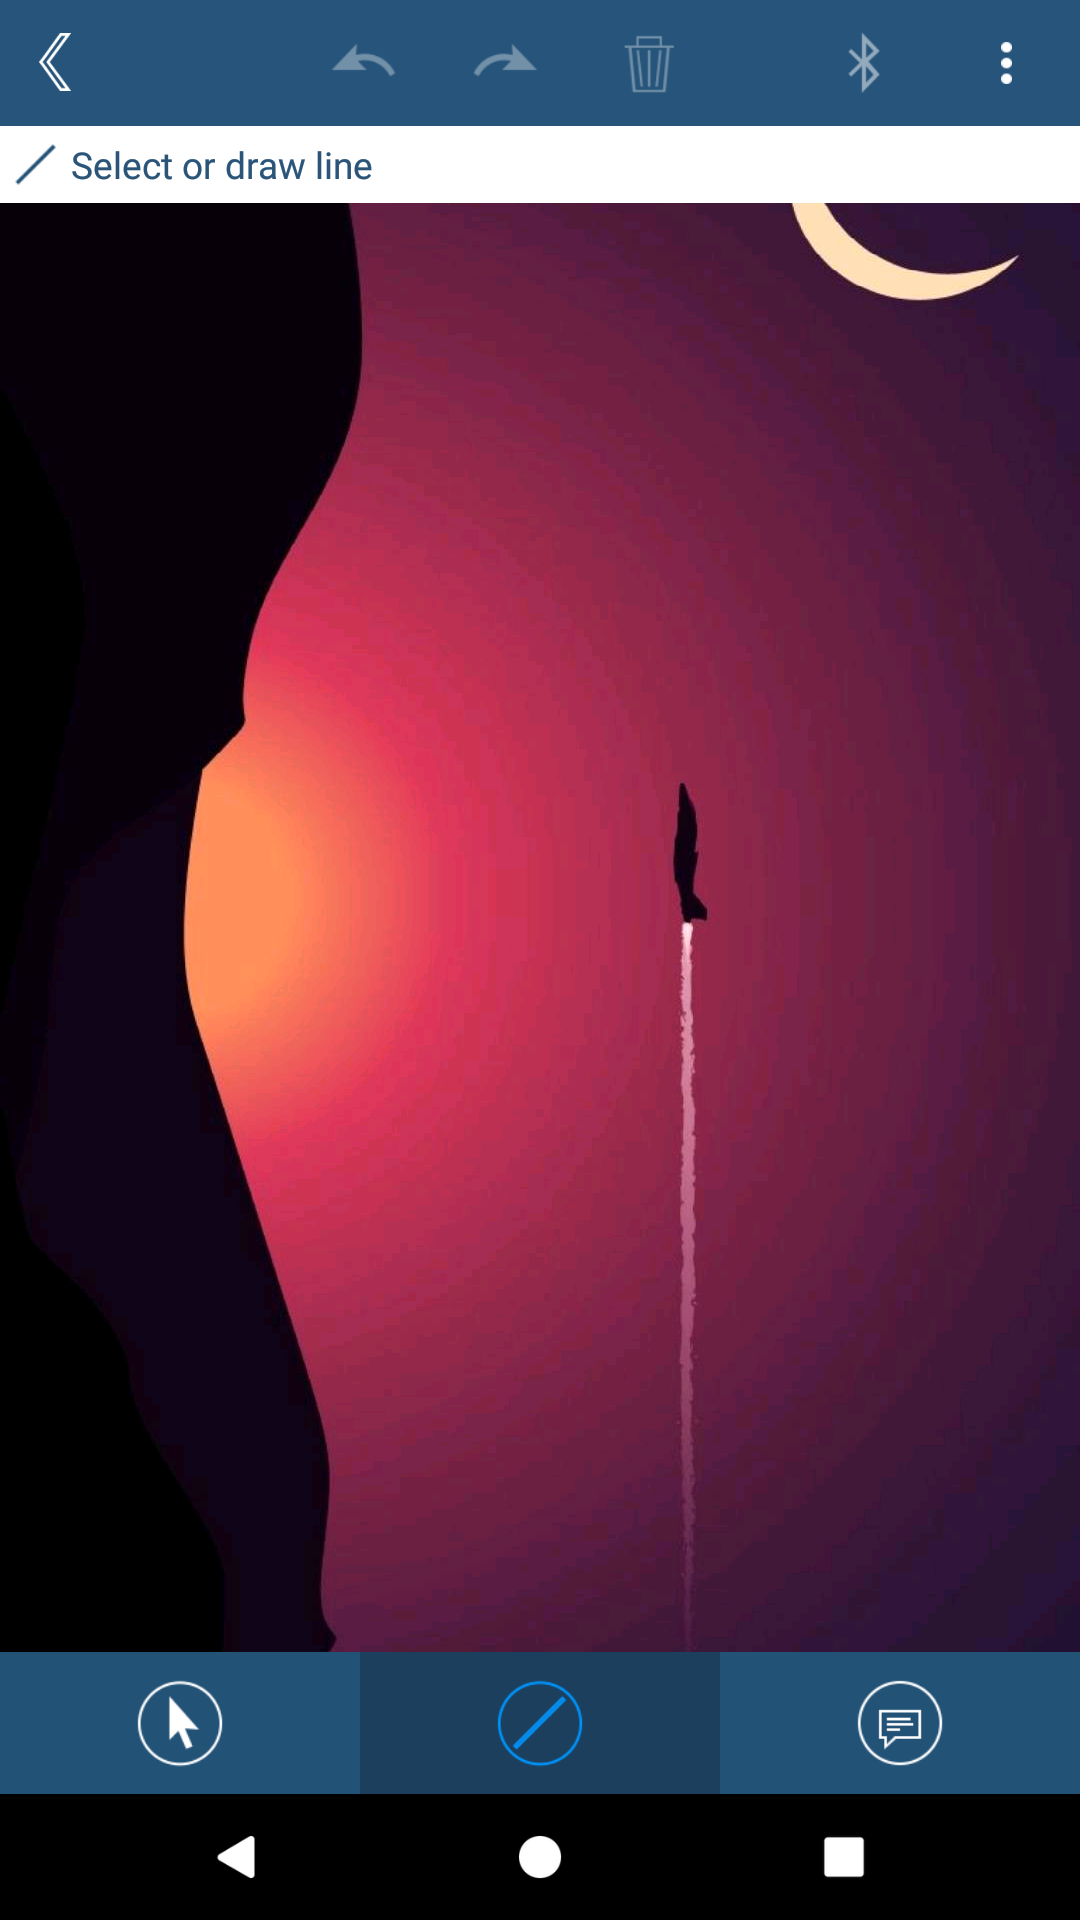
\includegraphics[keepaspectratio, width=0.9\linewidth]{bosch/portrait}
		\caption{App im Portrait-Modus}
		\label{fig:bportait}	
	\end{subfigure}
	~
	\begin{subfigure}[b]{0.5\textwidth}
		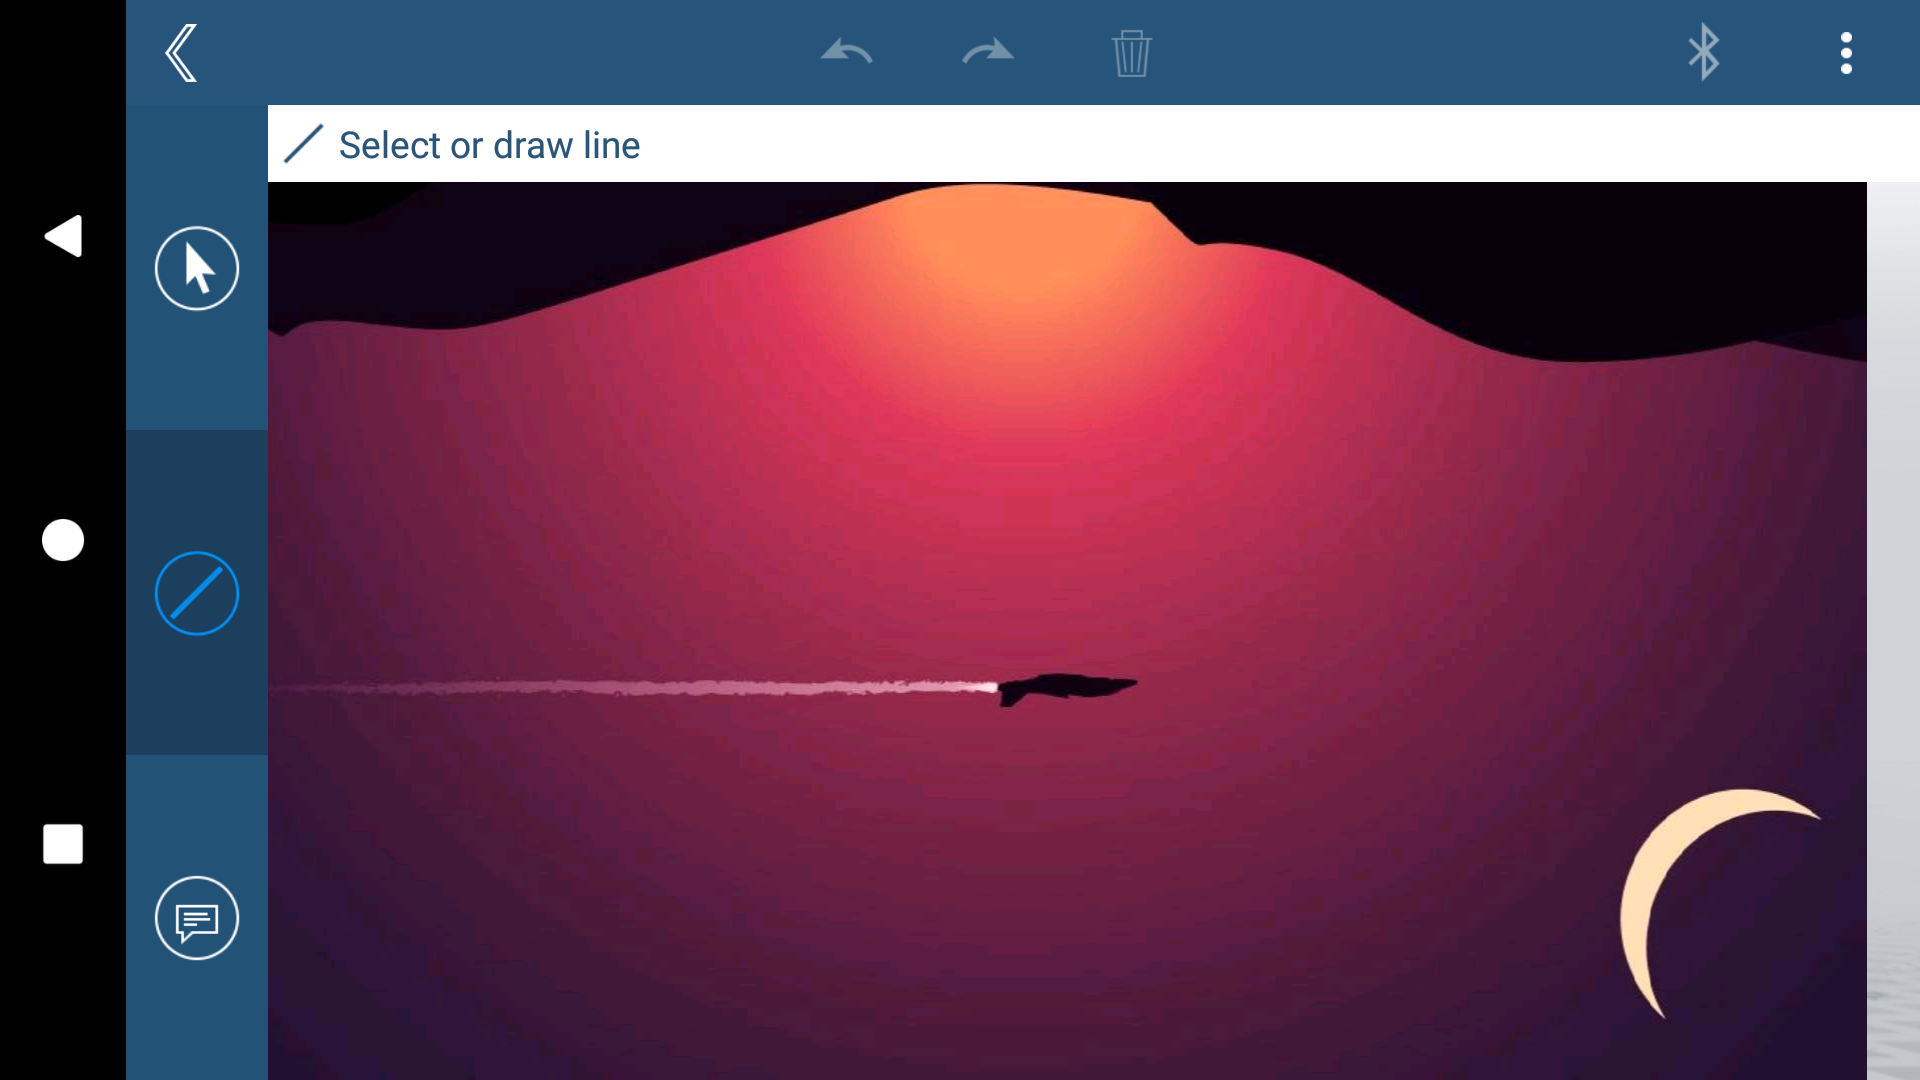
\includegraphics[keepaspectratio, height=0.7\linewidth]{bosch/landscape}
		\caption{App im Landscape-Modus}
		\label{fig:blandscape}	
	\end{subfigure}
	\caption{Bildschirmrotation Bosch-App}
	\label{fig:borientation}
\end{figure}

\subsection{Measures \& Sketch}

\textsc{Measures \& Sketch} von HERSTELLER, VERSION, RANKING \\

\begin{wrapfigure}{R}{0.4\textwidth}
	\includegraphics[keepaspectratio, width=0.4\textwidth]{measure_sketch/help}
	\caption{Hilfe-Overlay}
	\label{fig:mshelp}
\end{wrapfigure}

Auch diese App bedient sich eines Hilfe-Overlays beim ersten Start, überfordert den Benutzer jedoch mit zu viel Text. So erfüllt dieses Tooltip ihre Funktion als Hilfestellung nicht, sondern überfordert den Nutzer mit Text. Alternativ bietet sich auch bei dieser App wie in \autoref{fig:pmhelp} mit Icons zu arbeiten, sodass die Gedächtnisbelastung minimiert wird. \\

Die App kann als negativ-Beispiel bezüglich der Nielsen-Heuristiken betrachtet werden. Es gibt weder Undo- oder Redo-Button, noch wird in irgendeiner Weise hervorgehoben, welche Form aktuell ausgewählt ist. Dies führte beim Löschen oft zu Überraschungen. \\

 Außerdem unterstützt die App keinerlei Gesten zur Navigation im Bild. So lässt sich der abgebildete Bereich des Bildes weder zoomen, noch kann der Benutzer das Bild rotieren oder verschieben. Um Formen zu zeichnen bedient sich die App eine für den Benutzer unnatürliche Geste, denn hierzu muss der Nutzer gleichzeitig mit zwei Fingern die Form in die beiden gewünschten Richtungen ``aufziehen''. So fühlt sich der Zeichen-Prozess nicht nur unnatürlich an, sondern ist in der Größe der Form durch die Spannweite der Finger des Benutzers beschränkt. \\
 
 Zusätzlich schließt dies die Benutzung der App mit einer Hand aus, was Nielsen~\autoref{itm:16} klar widerspricht. Als Bildschirmausrichtung wird nur der Portrait-Modus unterstützt, was gerade die Bearbeitung von im Landscape aufgenommenen Bildern zu einer Herausforderung macht. \\

\section{Bewertung der Lösungsalternativen}

\todo{Punkte auf Konsistenz überprüfen}
\begin{sidewaystable}[ht]
	\centering
	\caption{Vergleich der Lösungsalternativen}
	\vspace*{10px}
	\label{tab:nielsen}
	\begin{tabular}{r|l|c|c|c|}
	\cline{2-5}
    	        				    &								& Photo Measures 	& Measuring Master 	& Measure \& Sketch \\ \cline{2-5} 
	Nach \cite{Nielsen:1994:UIM}	& \autoref{itm:1}				&       \po 		&    \po 			&       \xmark      \\ \cline{2-5} 
    	             				& \autoref{itm:2} 				&       \po  		&    \po  			&       \po		    \\ \cline{2-5}
    	             				& \autoref{itm:3} 				&       \xmark 		&    \po			&       \xmark      \\ \cline{2-5} 
    	             				& \autoref{itm:4} 				&       \po  		&    \po			&       \xmark      \\ \cline{2-5}
    	            				& \autoref{itm:5} 				&       \po  		&    \xmark			&       \xmark      \\ \cline{2-5} 
    	            				& \autoref{itm:6} 				&       \xmark 		&    \po  			&       \xmark      \\ \cline{2-5} 
    	             				& \autoref{itm:7} 				&       \po  		&    \xmark			&       \xmark      \\ \cline{2-5} 
    	             				& \autoref{itm:8} 				&       \nl  		&    \po  			&       \xmark      \\ \cline{2-5} 
    	             				& \autoref{itm:9} 				&       \po   		&    \po  			&       \nl	        \\ \cline{2-5} 
    	            				& \autoref{itm:10} 				&       \po  		&    \po 			&       \xmark      \\ \cline{2-5} 
    	             				& \autoref{itm:11} 				&       \po   		&    \po 			&       \xmark      \\ \cline{2-5} 
    	             				& \autoref{itm:12} 				&       \po   		&    \po 			&       \xmark      \\ \cline{2-5} 
    	             				& \autoref{itm:13}			 	&       \xmark  	&    \xmark			&       \xmark      \\ \cline{2-5} 
    	            				& \autoref{itm:14} 				&       \po   		&    \po  			&       \po		    \\ \cline{2-5}
    	            				& \autoref{itm:15} 				&       \po   		&    \xmark			&       \xmark  	\\ \cline{2-5}   
    	            				& \autoref{itm:16} 				&       \po   		&    \po  			&       \xmark      \\ \cline{2-5} 
    	             				& \autoref{itm:17} 				&       \po  		&    \po  			&       \xmark		\\ \cline{2-5} 
    	             				& \autoref{itm:18} 				&       \nl  		&    \nl 			&       \nl		    \\ \cline{2-5} 
	Eigene Kriterien 				& \autoref{itm:integration}		&      	\xmark		&    \xmark			&       \xmark      \\ \cline{2-5}
	    	         				& \autoref{itm:export}   		&      	\xmark		&    \xmark			&       \xmark      \\ \cline{2-5}

	    	             
	\end{tabular}
	\\
	\vspace*{10px}
	\begin{tabular}{l}
		\po~wird erfüllt \\
		\nl~wurde nicht berücksichtigt \\
		\xmark~wird nicht erfüllt
	\end{tabular}
\end{sidewaystable}

\clearpage
\section{Vorgehensweise bei Implementierung eigener Software-Lösung}

\todo{vielleicht eigene sections?}
\subsection{Human-Centered Design Process}
\citeauthor{Norman:2013} beschreibt in seinem Buch ``The Design of Everyday Things: Revised and Expanded Version'' zur Vorgehensweise bei der Lösung von Usability-Problemen unteranderem den ``Human-Centered Design Process'' \citep[Seiten 221--230]{Norman:2013}. 

\begin{figure}[h]
	\centering
	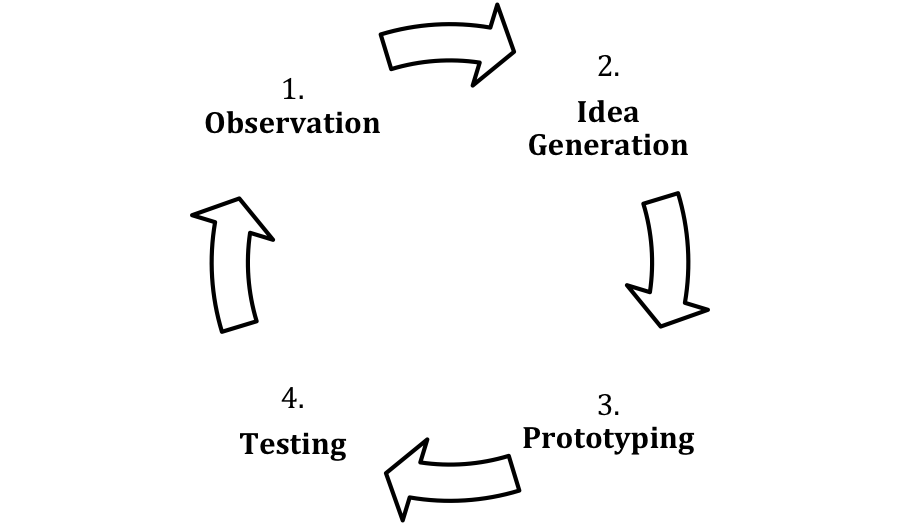
\includegraphics[keepaspectratio]{hcp}
	\caption{The Human-Centered Design Process}
	\label{fig:hcp}
\end{figure}

In \autoref{fig:hcp} sieht man die vier verschiedenen Phasen des Zyklus:
\begin{enumerate}
	\item Beobachtung (Observation) \label{itm:observation}
	\item Ideenfindung (Idea Generation) \label{itm:idea}
	\item Prototypenentwicklung (Prototyping) \label{itm:prototyping}
	\item Testen (Testing) \label{itm:testing}
\end{enumerate}

Eingangs werden in der Beobachtungs-Phase (Observation) Test-Personen ausgesucht, die möglichst nah an die wirklichen Ziel-Bedingungen kommen  und bei ihrer alltäglichen Arbeit beobachtet. Dies steigert die Wahrscheinlichkeit am Ende der Beobachtung möglichst aussagekräftige Einblicke in eventuelle Probleme dieser Zielgruppe zu bekommen. 

Anschließend werden in der Ideenfindungs-Phase (Idea Geneartion) möglichst viele Ideen zur Lösung der Probleme aus Phase 1 herausgearbeitet, welche in der dritten Phase (Prototyping)  in Form eines Mock-ups oder ersten Prototypen versucht gelöscht zu werden.

Um den ersten Durchgang des Zyklus abzuschließen bekommt in der vierten Phase (Testing) eine ausgewählte Menge an Test-Personen die Ergebnisse aus der Prototypenentwicklung vorgelegt. So können bis dahin unerkannte oder sogar neu erstandene Probleme gefunden werden, welche in die nächste Iteration des Design-Prozesses einfließen.

 Das Ziel ist es, den Prozess so lange zu wiederholen, bis sich optimaler-weise keine Usability-Probleme mehr aufzeigen.  \\
 
 \subsection{Die 8 Goldenen Regeln von Shneiderman}
 
\citeauthor{Shneiderman:2004} definieren in ihrem Buch ``Designing the User Interface: Strategies for Effective Human-Computer Interaction'' die sogenannten ``8 Goldenen Regeln des Interface Designs''.  Die acht Regeln lauten wie folgt:

\begin{enumerate}
	\item Bemühe Dich um Konsistenz (``Strive for consistency'')
	\item Erlaube erfahrenen Benutzern die Nutzung von Abkürzungen (``Enable fequent users to use shortcuts'')
	\item Biete informative Rückkopplung (``Offer informative feedback'')
	\item Biete ein klares Ende von Teildialogen an (``Design dialogs to yield closure'')
	\item Biete Fehlervermeidung und einfache Fehlerbehandlung an (``Offer error protection and simple error handling'')
	\item Erlaube eine einfach Rücknahme von Aktionen (``Permit easy reversal of actions'')
	\item Gib dem Benutzer die Kontrolle (``Support internal locus of control'')
	\item Minimiere Gedächtnisbelastung (``Reduce short-memory load'')
\end{enumerate} 


  \subsection{Iterativer Entwicklungsprozess}
    3 Iterationen jeweils Mitte Dezember, Januar und Februar \\
    Feedback in Form von Gitlab-Issues und Beobachten von Testpersonen (Usability-Experimente) \\
    1. Iteration (Dezember): App mit floating buttons (screenshots vorher-nachher)
    2. Iteration (Januar): App mit status bar (screenshots vorher-nachher)
    3. Iteration (Februar): App mit Help-Overlay \& verbesserter Statusbar (screenshots vorher-nachher)
  \subsection{DIN und ISO-Normen}
  \subsection{Material Design-Guidelines}
  \subsection{ABC-Modell}
  \subsection{Gesture-Support (papers)}
    Zoom-Area und Panning am besten geeignet um Content auf kleinen Displays darzustellen \\


  
1